\section{Estrutura}

\par Baseado nos requisitos estruturais apresentados no PC01 e atualizados na tabela \ref{tab:Requisitos de Estrutura}, a solução de estrutura foi desenvolvida.

\begin{table}[H]
\centering
\begin{tabular}{ | m{2cm} | m{12cm}| } 
 \hline
 \textbf{Requisito} & \begin{center}\textbf{Descrição}
   
 \end{center} \\ 
 \hline
 RFEST01 & Ser de uso intuitivo para o usuário.\\
 & \\
\hline
 RFEST02 & Uma estrutura física compacta e portátil, que dê suporte aos componentes internos da estação. \\
 \hline
 RFEST03 & Material leve e resistente, capaz de proteger os componentes internos da estação de eventuais impactos e intempéries provenientes do ambiente e de seu deslocamento. \\
  \hline
RFEST04 & Uma segunda estrutura física compacta e portátil, voltada para o armazenamento do sistema de abastecimento. \\
\hline
RFEST05 & Ter um sistema de transmissão de torque do atuador para a válvula-esfera do sistema de abastecimento. \\
\hline
RFEST06 & Proteger o sistema eletrônico e não gerar interferência neste.  \\
\hline
RFEST07 & Estrutura interna acessível e de fácil manutenção. \\
\hline
RFEST08 & Sistema de abastecimento baseado nos componentes definidos pelo cliente. \\
\hline
\end{tabular}
\caption{Requisitos de Estrutura}
\label{tab:Requisitos de Estrutura}
\end{table}

\begin{figure}[!h]
	\centering
	\label{bateria_maleta}
		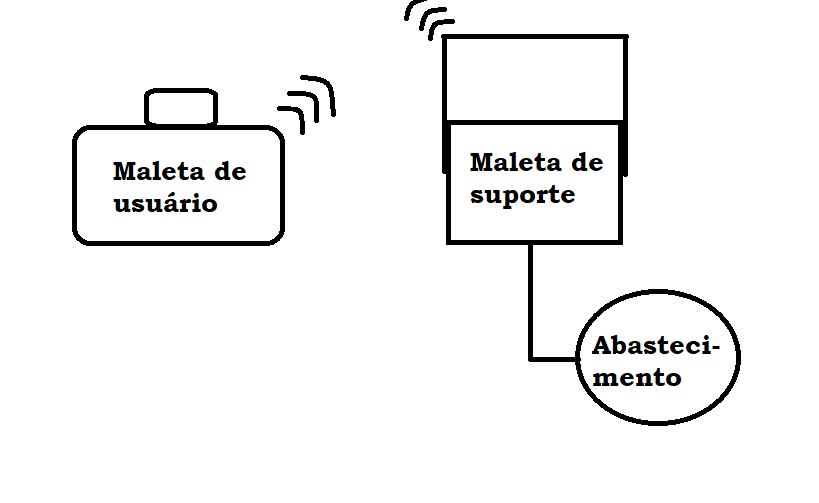
\includegraphics[width=0.7\textwidth]{figuras/estrutura.png}
	\caption{Solução estrutural}
	\label{soluçao_estrut}
	\end{figure}

\par O RGS necessita que todo o seu sistema seja portátil e suficiente para configurar e apoiar as missões de foguetes da CTR. Assim, durante sua concepção estrutural, o principal foco da equipe foi a mobilidade e a robustez para adequação às condições ambientais encontradas nos potenciais locais de lançamento e teste de foguetes. Por isso nossa solução estrutural deve ser equipada com todos os instrumentos necessários para o suporte eletrônico e de software responsáveis por rastrear e comandar o foguete durante o lançamento.

\par Dessa forma, nossa solução se divide em três frentes. A primeira é a maleta de usuário, onde ficarão os componentes eletrônicos e a interface de usuário de software (\ref{maleta_01}). Depois tem-se a maleta de suporte, responsável por abrigar os componentes para o abastecimento e a ignição do foguete à distância (\ref{maleta_02}). E, por fim, tem-se o sistema de abastecimento e ignição em si com seus componentes em uso integrados a outras partes do projeto (\ref{abastecimento}). Na figura \ref{soluçao_estrut} pode-se ver como o trabalho estrutural foi dividido.


\subsection{Maletas}

\par A solução estrutural inicial era de desenvolver apenas uma estrutura em formato de maleta, visando que ela fosse o bastante para o uso e carregamento de toda a solução. Porém, depois foi visto que a solução proposta demandaria do cliente o uso de um cabo de energia, muito superior aos comerciais, se tornando um empecilho para a usabilidade do produto. Além de que um cabo elétrico de grandes dimensões possui perda ao longo de sua transmissão, assim foi optado por desenvolver uma solução totalmente segura e sem fios para o conjunto de controle e de abastecimento. 

\par Fazendo-se então necessária a construção de uma segunda estrutura para comportar e transportar os elementos de abastecimento de modo que esse fique perto da base de lançamento, enquanto a outra estrutura fica em uma distância segura com o usuário.

\begin{figure}[!h]
	\centering
	\label{bateria_maleta}
		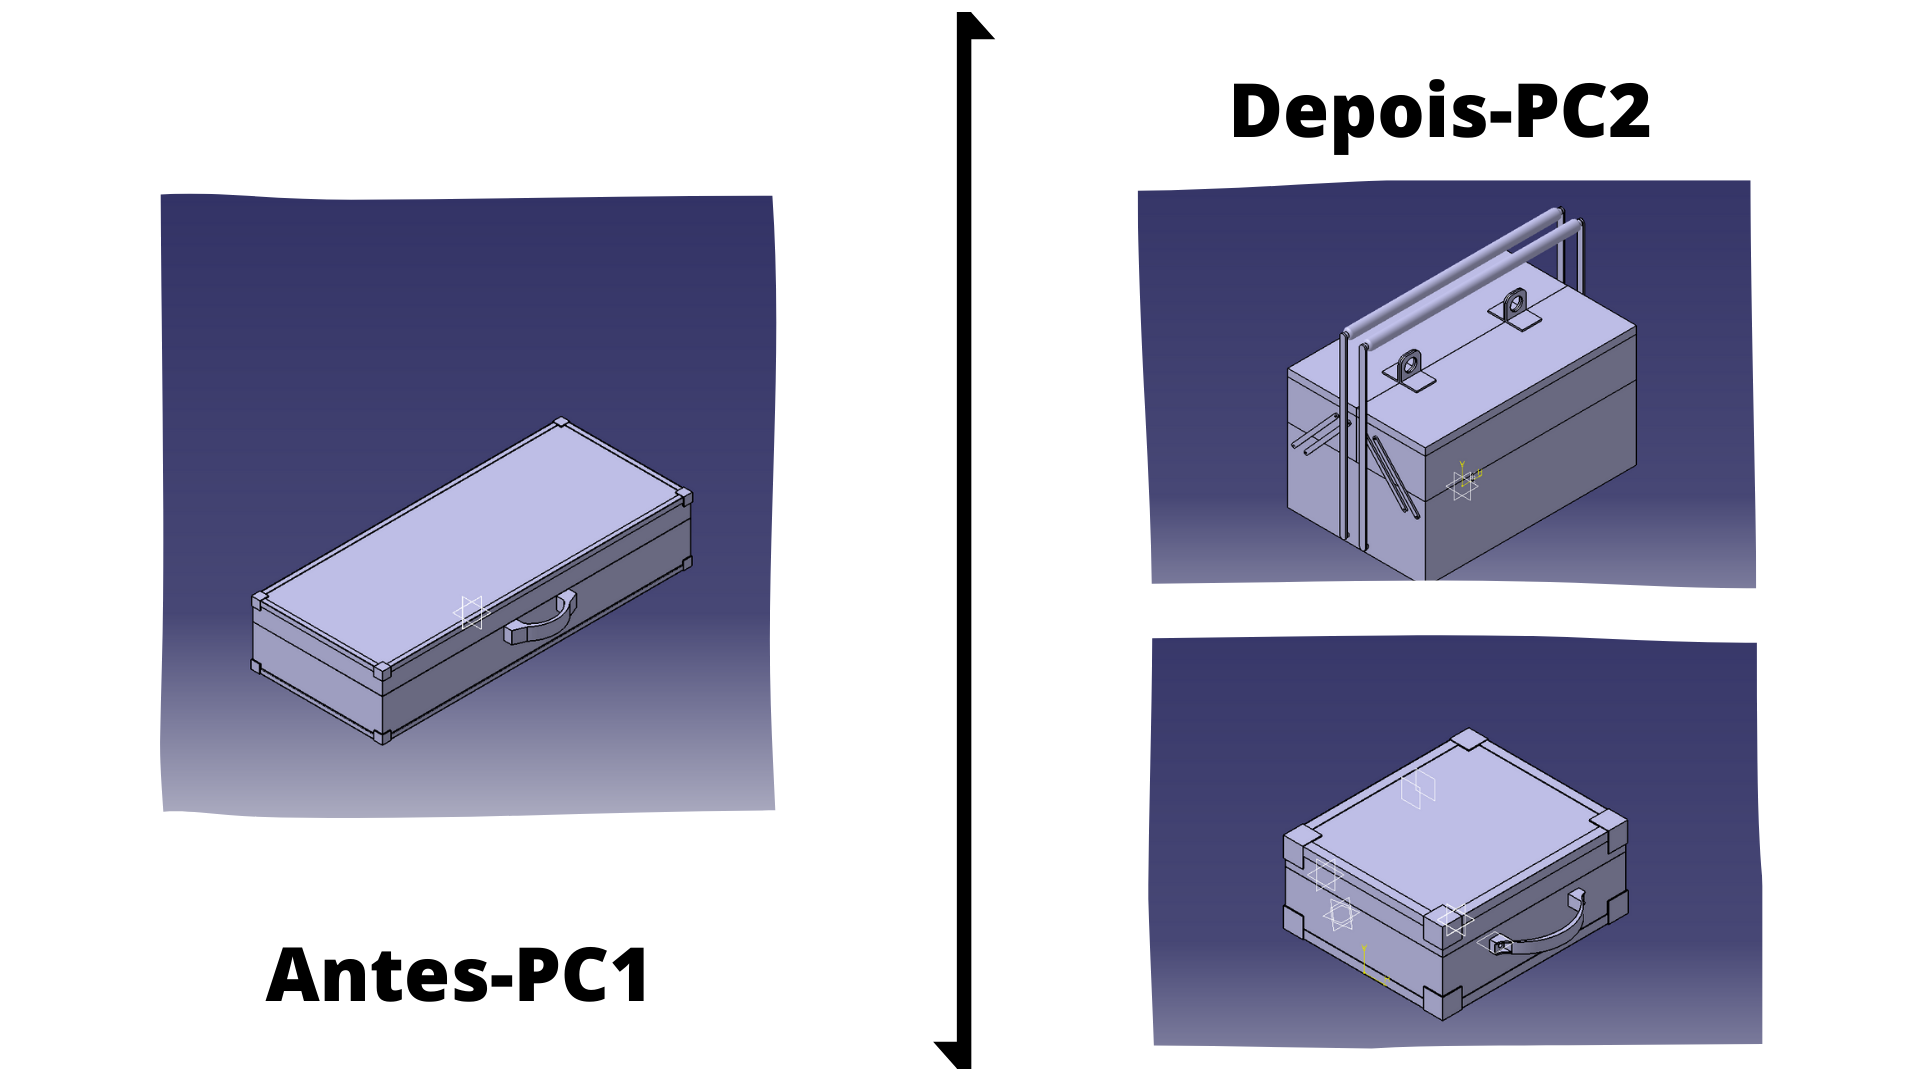
\includegraphics[width=1\textwidth]{figuras/antes_depois.png}
	\caption{Solução no PC1 e solução no PC2}
	\label{antes_depois}
	\end{figure}

\subsubsection{Especificações de materiais}
\label{sub:Especificações de materiais}

\par Durante a seleção de materiais, é necessária uma sistematização que permita analisar a vasta possibilidade de combinação de materiais que podem constituir determinado produto a fim de extrair um candidato vencedor, que cumpra com maior eficiência possível os requisitos da aplicação \cite{walterconteudo}.

\par Antes de apresentar a lista em si, é necessário evidenciar as características desejáveis para as estruturas que serão utilizadas na solução. Durante a etapa de escolha do material a ser utilizado, nem sempre é possível contemplar satisfatoriamente todos os aspectos necessários para aquela determinada finalidade. Por isso, tais aspectos são dispostos em ordem de relevância para o projeto, para que a escolha do material seja feita com embasamento teórico dentro da necessidade real do protótipo. 

\begin{enumerate}
    \item O fator mais relevante para a caixa da \textit{ground station} é o correto funcionamento no local de lançamento. A caixa deve estabelecer, por meio de ondas eletromagnéticas, comunicação mútua com o foguete e com o sistema de abastecimento de propelente durante todas as etapas de lançamento. Portanto, o material escolhido \textbf{não deve gerar interferência} nos sistemas de comunicação. 
    \item A usabilidade e a ergonomia vem a seguir, responsáveis por garantir que o usuário consiga ler, de forma clara e precisa, todos os parâmetros relevantes para a missão e que o auxiliará na tomada de decisão. Assim, \textbf{o material utilizado deve ser moldável} para que embarque os componentes necessários e os disponha de maneira adequada, respeitando as suas diferentes geometrias.
    \item O \textbf{custo} é o terceiro fator mais relevante, uma vez que a viabilidade de fabricação do protótipo está diretamente relacionada com seu valor final. Além do material ser acessível do ponto de vista financeiro, é desejável que ele permita agilidade em sua construção, dado que um material difícil de ser trabalhado pode gerar mais horas de trabalho, o que resulta no aumento do valor total da mão-de-obra e, por consequência, aumento do valor final do protótipo.
    \item Como quarta prioridade, a caixa deve ser resistente de maneira que eventuais quedas ou impactos com outros objetos não venha a interferir o seu correto funcionamento. Materiais com boa \textbf{resistência mecânica} podem contemplar tal característica.
    \item Por fim, a portabilidade se faz necessária devida à utilização da caixa ocorrer em lugares de acesso restrito. Logo, a caixa deve ser \textbf{leve e compacta} para facilitar o seu transporte.
\end{enumerate}

\par Visto os aspectos desejáveis, é apresentado a seguir o estudo de possíveis materiais a serem utilizados no protótipo, bem como a escolha final de uso.

\begin{itemize}
    \item \textbf{\textit{Medium Density Fiberboard} - MDF}
     \par O MDF é um material fabricado a partir da aglutinação de fibras de madeira com resina sintética – sendo as mais utilizadas à base de ureia formaldeído, tanino formaldeído e melamina ureia formaldeído –  posteriormente submetidas à prensagem em altas temperaturas  \cite{gomes}.  Sua composição permite que ondas eletromagnéticas possam fluir através dela.
     
    \par Sua superfície é plana e lisa, oferece alta usinabilidade para encaixar, entalhar, cortar, parafusar, perfurar e moldurar, além de reduzir o uso de tintas, vernizes e ótima aceitação de revestimentos \cite{CAMPOS}.
    
    \par O custo varia de acordo com a espessura da chapa. O valor do metro quadrado de uma chapa de 3 mm é R\$36,81. Já uma chapa de 6 mm custa R\$62,50 o metro quadrado.  Por possuir boa trabalhabilidade \cite{eleoterio2000propriedades}, o processo de construção pode apresentar satisfatória rapidez.  
    
    \par As características mecânicas específicas do material variam de acordo com o tipo de fibra e resina utilizadas. Em geral, são vantagens do MDF a alta relação entre resistência mecânica e massa específica, homogeneidade e ausência de defeitos como nós e desvios de grão \cite{eleoterio2000propriedades}. 
    
    \par De acordo com Silva e Gonçalves \cite{da2007avaliaccao}, os MDF são projetados para serem fabricados com densidades entre 0,5 e 0,8 $g/cm^3$. 
    
    \par Na tabela \ref{tab:mdf} é apresentado algumas das principais propriedades físicas e mecânicas de painéis MDF confeccionados com madeira de \textit{Eucalyptus grandis}.
    
\begin{table}[h]
\centering
\begin{tabular}{|l|l|}
\hline
Densidade              & 0,695 $g/cm^3$ \\ \hline
Módulo de elasticidade & 3776 $MPa$ \\ \hline
Módulo de ruptura      & 36,1 $MPa$ \\ \hline
Resistência a tração   & 1,01 $MPa$ \\ \hline
\end{tabular}
\caption{Propriedades do MDF}
\label{tab:mdf}
\end{table}

    \item \textbf{Polímero Reforçado com Fibra de Vidro - PRFV}
    
    \par É um material composto por uma matriz de resina sintética termofixa, como a Resina Epóxi, reforçada com estreitos filamentos flexíveis de vidro, cujo principal constituinte é a sílica \cite{pierin2005estudo}. O PRFV não gera interferência na comunicação com os sistemas. 
    
    \par Possui razoável manuseabilidade, pode ser cortado, perfurado e moldado, porém caso a caixa seja composta por várias peças o encaixe entre elas pode dificultar o processo de montagem.    
    
    \par O processo de fabricação é lento pois é necessária a fabricação do PRFV em si, ou seja, não é vendido o PRFV pronto para uso e sim os filamentos de vidro e a resina. Além disso, o PRFV deve ser confeccionado em um molde que deve ser previamente fabricado com o formato da peça final. O custo de material suficiente para produzir um metro quadrado de PRFV é de R\$52,90.  
    
    \par De acordo com Lin et al (1996), conforme citado por Pierin \cite{pierin2005estudo}, os PRFV exibem alta resistência mecânica, porém problemas de deformabilidade e instabilidade, devido à sua baixa elasticidade e rigidez, são os maiores inconvenientes deste material. 
    
    \par De acordo com CALLISTER JR. \cite{callister2000ciencia}, a densidade do PRFV varia entre 1,5 $g/cm^3$ podendo chegar até próximo de 3 $g/cm^3$ dependendo dos materiais utilizados.
    
    \item \textbf{Polímero Reforçado com Fibra de Carbono - PRFC}
    \par Similar ao PRFV, o PRFC utiliza como reforço fibras compostas principalmente de carbono que resultam da pirólise de fibras plásticas, como a poliacrilonitrila (PAN). 
    
    \par O processo de fabricação do PRFC é análogo ao processo de fabricação do PRFV. O material para produzir um metro quadrado PRFC custa R\$421,43.
    
    \par Segundo Galli \cite{galli2016caracterizaccao} as fibras de carbono são normalmente empregadas em aplicações que requerem elevadas propriedades mecânicas (alta resistência mecânica e alto módulo de elasticidade) associadas a uma baixa densidade.
    
    \begin{table}[h]
\centering
\begin{tabular}{|l|l|}
\hline
Densidade              & 1,78 $g/cm^3$ \\ \hline
Módulo de elasticidade & 380 $MPa$ \\ \hline
Módulo de ruptura      & 124,5 $MPa$ \\ \hline
Resistência a tração   & 102,9 $MPa$ \\ \hline
\end{tabular}
\caption{Propriedades do PRFC}
\label{tab:PRFC}
\end{table}
    
    \item \textbf{Poli Ácido Lático - PLA}
    
    \par O PLA é um polímero termoplástico feito através da extração do milho, trigo ou cana de açúcar passando por várias etapas de produção. Sua composição permite o correto funcionamento dos sistemas de comunicação. 
    
	\par O PLA é um material comumente usado em prototipagem rápida onde uma impressora 3D deposita o material partindo de dados provenientes de sistemas de desenho assistido por computador (CAD). Sua alta fluidez e baixa contração durante o processo de extrusão permite a produção de peças com alta precisão dimensional e bom acabamento superficial.
	
	\par O filamento de PLA para impressão 3D tem valor médio de R\$140,00 o kg com a possibilidade e facilidade de poder encontrá-los em diversas cores. O valor de processamento do PLA para projetos com baixas unidades é muito elevado, tornando inviável seu processamento por injeção ou \textit{vacuum forming} e impressão 3D. 
	
	\par De acordo com Simões et al. \cite{simoes2009mechanical}, o PLA é um material rígido e resistente, difícil de deformar ou flexionar, possui alta dureza, que o torna com baixa resistência ao impacto. É um material indicado para produção de protótipos que não sejam submetidos às condições de altos esforços mecânicos, atritos ou altas temperaturas.


    \begin{table}[h]
\centering
\begin{tabular}{|l|l|}
\hline
Densidade              & 1,24 $g/cm^3$ \\ \hline
Módulo de elasticidade & 2690 $MPa$ \\ \hline
Módulo de ruptura      & 53,32 $MPa$ \\ \hline
Resistência a tração   & 50,0 $MPa$ \\ \hline
\end{tabular}
\caption{Propriedades do PLA}
\label{tab:PLA}
\end{table}

    \item \textbf{Acrilonitrila Butadieno Estireno - ABS}
    
    \par Para  Vossen  \cite{vossen2009nanocompositos},  o  ABS é  um  termoplástico  que  consiste em uma  fase  de  borracha  (butadieno)  dispersa  em  uma  matriz de  SAN  (copolímero  de  acrilonitrila  Estireno),  também denominado terpolímero.
    
	\par A acrilonitrila confere estabilidade ao calor e resistência química e à flexão; o butadieno é responsável pela resistência ao impacto e tenacidade; já o estireno por sua vez é responsável pelo brilho, rigidez e fácil processamento. Devido à suas propriedade e baixo custo o ABS se tornou um material bastante utilizado por várias indústrias. O ABS pode ser Processado por injeção, extrusão e sopro.
	
	\par O valor do ABS depende da forma em que você o deseja, o kg do ABS granulado custa em média R\$ 16,80 já o kg do filamento (399 m) de ABS para impressão varia de R\$50,00 a R\$100,00. O valor de processamento do ABS para projetos com baixas unidades é muito elevado, tornando inviável seu processamento por injeção ou \textit{vacuum forming} e impressão 3D.
	
	\par Assim as propriedades do ABS dependem do teor de cada componente, mas em geral o ABS apresenta boa resistência térmica e ao impacto, alta estabilidade dimensional, alta rigidez, alta dureza, baixa absorção de umidade, etc. \cite{junior2014aspectos}

    \begin{table}[h]
\centering
\begin{tabular}{|l|l|}
\hline
Densidade              & 1,05 $g/cm^3$ \\ \hline
Módulo de elasticidade & 1335,9 $MPa$ \\ \hline
Módulo de ruptura      & 29,0 $MPa$ \\ \hline
Resistência a tração   & 62,0 $MPa$ \\ \hline
\end{tabular}
\caption{Propriedades do ABS}
\label{tab:ABS}
\end{table}

\end{itemize}

\par A partir dos dados apresentados para os diferentes materiais, é possível chegar às seguintes conclusões: os materiais selecionados para o estudo são caracterizados por não gerarem interferência; assim, o próximo aspecto a ser analisado é o usinabilidade e geometrias que o material pode assumir com poucos processos. Nesse quesito, os materiais com fibras se tornam menos atraentes por sua complexa usinabilidade. Já no quesito custo os materiais mais comerciais possuem melhor custo beneficio como é o caso do MDF. Porém, as características mecânicas e físicas são o fator decisivo para a escolha do material, com a menor densidade entre os materiais selecionados e o maior modulo de elasticidade o MDF, se saiu na frente nos dois últimos quesitos analisados. Apesar da sua baixa resistência a tração, o fato de o sistema desenvolvido não estar sujeito a esse tipo de carga faz que ele se torne ainda mais atrativo. Logo, o material escolhido para a confecção do protótipo é o \textbf{MDF}.

\par Walter sinaliza que a dinâmica de Seleção de Materiais e Processos de Fabricação devem ser flexíveis a ponto de permitir sua utilização em etapas desde o \textit{Design} Conceitual ao Projeto para Manufatura \cite{walterconteudo}. 

\par Tratando-se de um projeto de engenharia, foi definida a escolha de mais de um material, já que suas partes possuem funções diferentes. Assim a carcaça da caixa será feita em com um material de revestimento (cf. \ref{revestimento}), o que permite um acabamento melhorado e uma proteção em caso de eventual contato com líquidos. Enquanto que os componentes estruturais serão feitos em MDF feito de madeira de eucalipto, visto que a mesma segue o enquadramento para construção de painéis de uso estrutural determinado pela especificação NBR 15316-2 \cite{}. Assim combinando diferentes materiais, tem-se uma diminuição dos custos de produção, diminuição do peso e aumento das propriedades mecânicas se comparado aos polímeros.

\subsubsection{Material para revestimento da caixa}
\label{revestimento}

\par Para aumentar a resistência do material que forma as estruturas da estação de controle, recomenda-se o seu revestimento com material polimérico (i.e. borracha), de modo a aumentar sua resistência à abrasão, impacto, cortes e pressão. Em aplicações industriais, alguns desses polímeros são desenvolvidos para ser aplicados em condições extremas, a temperaturas muito altas ou em locais com presença de ácidos concentrados, o que foge do escopo do uso no projeto, de proteger a estação de intempéries ambientais e a choques mecânicos moderados, ou seja, queda de uma altura não superior a de uma pessoa carregando a maleta nas mãos: 1 a 1,5 m.

\begin{itemize}
    \item \textbf{Borracha de Etileno Propileno Terpolímero - EPDM }
    \par Material bastante usado para resistência térmica, mas também por sua dureza e por sua impermeabilidade à água.
    \item \textbf{Borracha de Estireno Butadieno - SBR} 
    \par Boa resistência à abrasão e resistência moderada a agentes atmosféricos (luz solar, oxigênio). Baixa resistência a ácidos fortes, solventes e a altas temperaturas (acima de 85ºC), o que extrapola a usabilidade esperada do material.
    \item \textbf{Borracha de Poliisopreno - IR}
    \par Propriedades muito próximas a da borracha natural. Grande resistência a abrasão, rasgo, mas baixa resistência a agentes atmosféricos (luz solar, oxigênio), que afetam seu envelhecimento.

\begin{table}[h!]
\centering
\begin{tabular}{|l|l|l|l|}
\hline
Propriedade & EPDM & SBR & IR \\ \hline
Dureza Shore A & 40-90 & 30-95 & 15-100 \\ \hline
Tensão de Rotura (MPa) & 7-18 & 7-21 & 15-25 \\ \hline
Resistência elétrica (ohms/cm$^2$) & 2 x 10$^{16}$ & 10$^{15}$ & 10$^{15}$ \\ \hline
Limites de temperatura (ºC) & -55 a 130  & -45 a 85 & -50 a 80 \\ \hline
Preço (R\$/m$^2$) & 140,00 & 80,00  & 100,00  \\ \hline
\end{tabular}
\caption{Propriedades material de revestimento}
\label{tab:revestimento}
\end{table}

\end{itemize}

\par A partir dos dados apresentados na tabela \ref{tab:revestimento} é possível ver que o material para revestimento com o melhor custo beneficio é o \textbf{SBR}, assim esse se torna o material escolhido para o revestimento. 

\subsubsection{Maleta 01 - GCS}
\label{maleta_01}
A maleta GCS é responsável por enviar o sinal de lançamento do foguete e colher os dados de telemetria deste. Dessa forma, ela tem que armazenar alguns componentes essenciais para que consiga realizar essa função e o usuário consiga analisar e colher os dados obtidos. Para armazenar todos esses componentes, foi pensado em uma maleta com \textit{design} mais robusto, porém, compacta. Suas especificações podem ser verificadas no Apêndice \ref{Drafts_do_projeto}.
\par Como pode ser observado na figura \ref{fig:Render Maleta GCS}, em sua base ficarão armazenados os componentes eletrônicos e de energia, tais como fontes, baterias, reguladores, etc. Ainda em sua base, para proteger os componentes eletrônicos e o usuário tem-se um fundo falso que serve como meio de acesso aos componente eletrônicos para manutenções e serve também de nicho para o teclado. Já em sua parte superior, a maleta conta com um outro fundo falso que permite acesso à tela de 9" e à base da antena.

\begin{figure}[H]
    \centering
        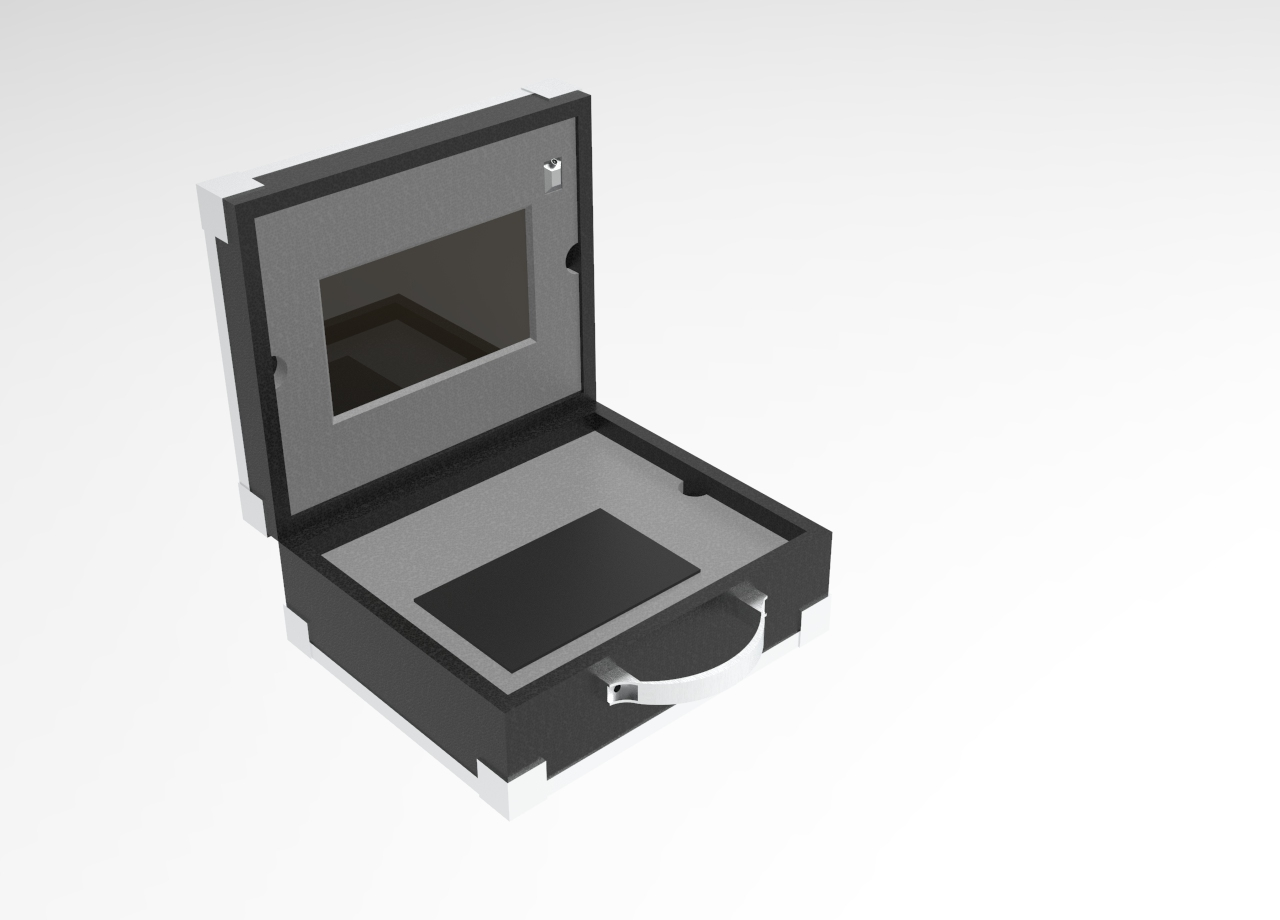
\includegraphics[width=\linewidth]{figuras/Render Maleta GCS.jpg}
    \caption{\label{fig:Render Maleta GCS} Maleta 01 - GCS}
\end{figure}

\par A disposição dos equipamentos eletrônicos, bem como o interior da base da GCS, podem ser observados na figura \ref{fig:Disposicao dos Componentes}.

\begin{figure}[H]
\centering
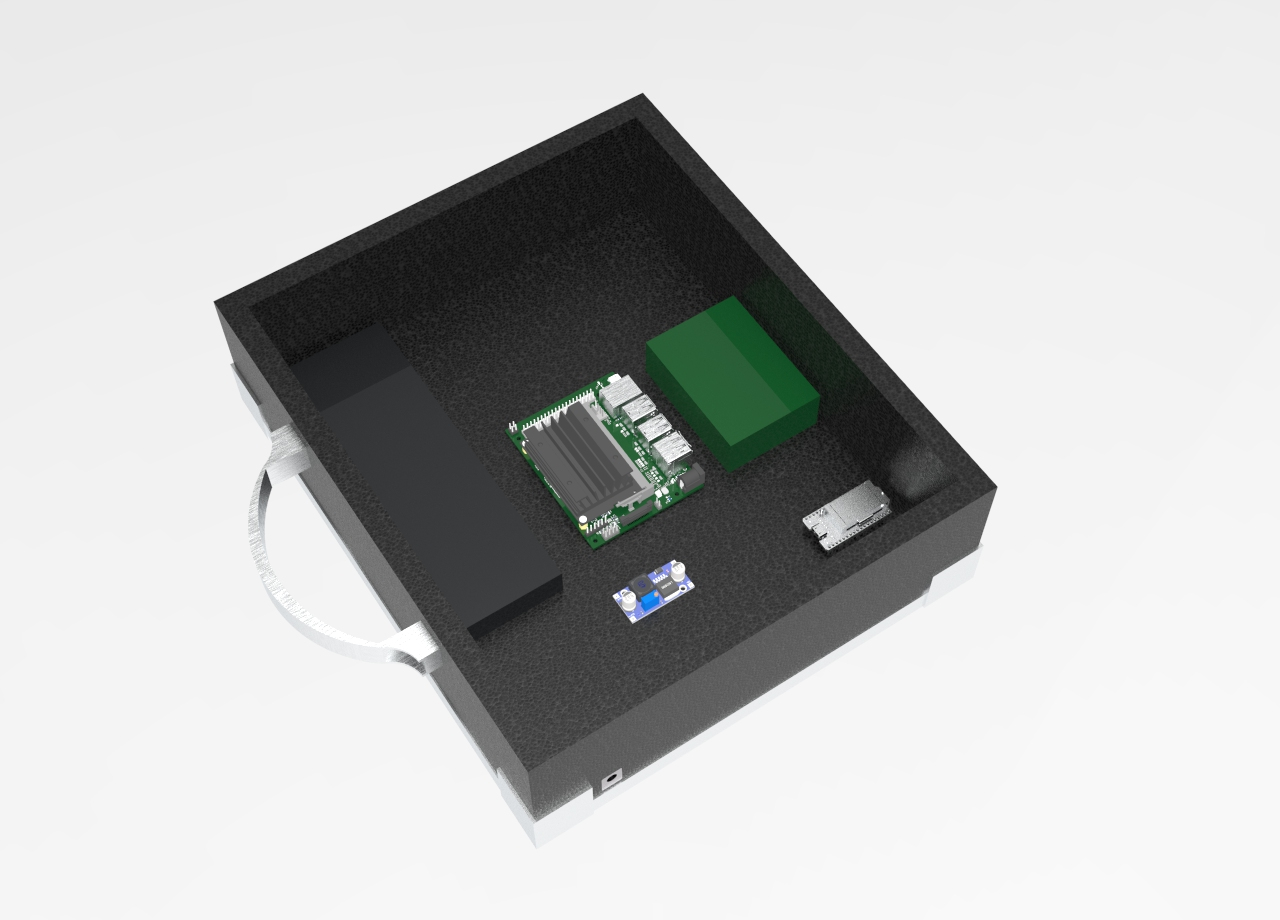
\includegraphics[width=0.65\textwidth]{figuras/Disposicao dos componentes.16.jpg}
\caption{Disposição dos equipamentos eletrônicos}
\label{fig:Disposicao dos Componentes}
\end{figure}

\par O peso da maleta GCS será de aproximadamente 4,539 kg. Essa estimativa foi realizada utilizando a ferramenta \textit{Measure Inertia} do software CATIA. Od dados obtidos no programa podem ser observados na  figura \ref{fig:PesoMGCS}.

\begin{figure}[H]
\centering
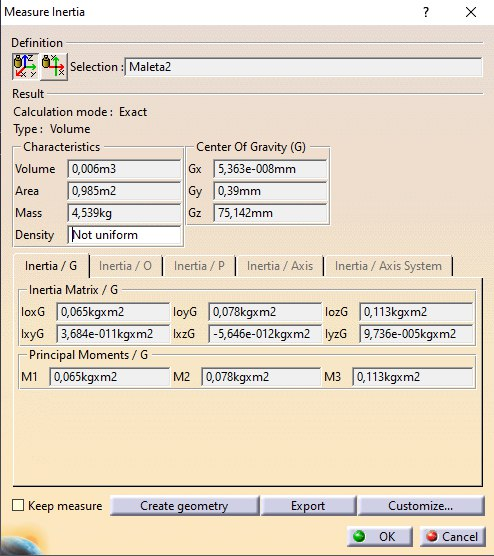
\includegraphics[width=0.65\textwidth]{figuras/PesoMGCS.jpg}
\caption{Resultados obtidos para a estimativa de peso da maleta GCS}
\label{fig:PesoMGCS}
\end{figure}

\subsubsection{Maleta 02 - Abastecimento}
\label{maleta_02}
A maleta de abastecimento tem como função transportar os atuadores, as válvulas, a mangueira de abastecimento e a bateria que proporcionará a energia necessária para o acionamento dos mesmos. Dessa forma, a maleta teve seu design inspirado em uma caixa de ferramentas. 
\par A maleta possuirá dois níveis. A base irá acomodar a mangueira e a bateria, fazendo que este seja o espaço com maior área útil na maleta (430x280x150 mm). Já o nível superior é composto por duas áreas de armazenamento simétricas (430x140x80 mm), com o objetivo de acomodar os motores e as válvulas como pode ser observado na figura \ref{fig:Render Maleta Alimentacao}. É possível observar as especificações para a produção da maleta no Apêndice \ref{Drafts_do_projeto}.

\begin{figure}[H]
\centering
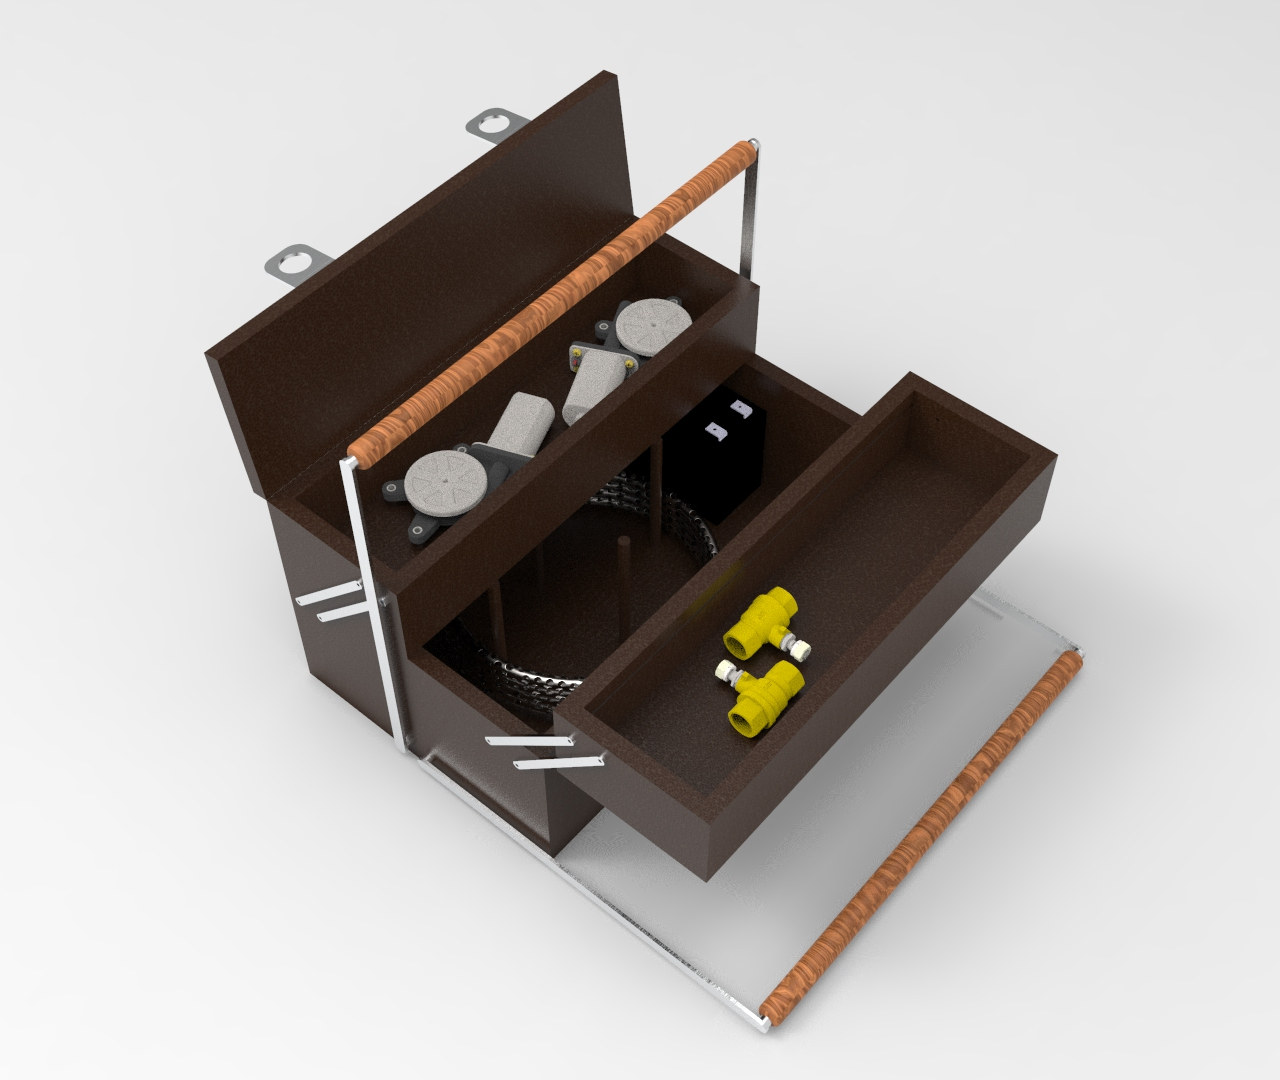
\includegraphics[width=0.9\textwidth]{figuras/Render Maleta Alimentacao.jpg}
\caption{Maleta 02 - Abastecimento}
\label{fig:Render Maleta Alimentacao}
\end{figure}

\par Na figura \ref{fig:PesoMA} é possível observar que o peso estimado para a maleta de abastecimento foi de 8,474 kg. O peso desta maleta foi estimado por meio da ferramenta \textit{Measure Inertia} do software CATIA.

\begin{figure}[H]
\centering
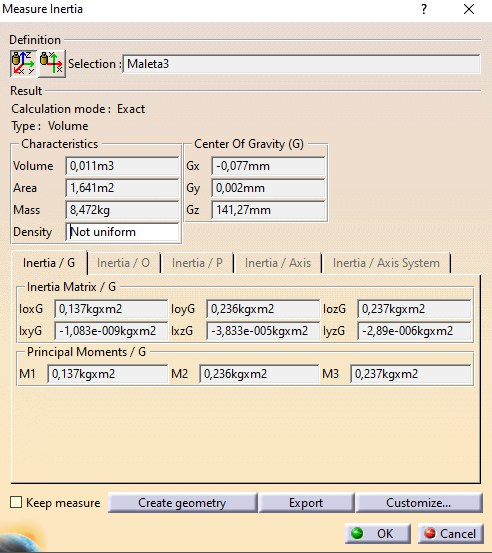
\includegraphics[width=0.7\textwidth]{figuras/PesoMA.jpg}
\caption{Resultados obtidos para a estimativa de peso da maleta GCS}
\label{fig:PesoMA}
\end{figure}

\subsubsection{Simulações de Impacto}

Tanto a maleta da estação de controle quanto a maleta do sistema de alimentação são estruturas que receberão pouca ou nenhuma carga (exceto o próprio peso) durante o seu funcionamento, ou mesmo o seu transporte. Porém, durante sua utilização, é possível que essas estruturas sofram algum impacto, em particular um impacto resultante de uma queda durante seu carregamento pelo usuário, ou a partir de uma mesa durante o seu uso. Nesse sentido, foi feita uma simulação, pelo Método de Elementos Finitos (FEM), com  uso do software Ansys, dessa situação.
\par Para a realização dessa simulação, foi considerada uma situação em que ambos os objetos atingem o solo a partir de uma condição inicial de repouso ($v_0 = 0$), em queda livre por uma altura $h = 1m$, sofrendo aceleração gravitacional constante de $g = 9,81 m/s^2$. Utilizando-se da equação de Torricelli \cite{hughd.young;rogera.freedman2008}:
\begin{equation}
    v^2 = v_0^2 + 2gh
\end{equation}
chegamos à velocidade a qual o objeto chega ao tocar o solo ($v = 4,4229 m/s$), velocidade esta que servirá de \textit{input} para a simulação.
\par A geometria utilizada para a simulação considerou as dimensões escolhidas para o desenho final de ambas as estruturas, desconsiderando seus componentes internos, uma vez que se visa a análise do material escolhido para a estrutura (MDF), bem como para o revestimento (SBR). Ambos os objetos foram colocados em colisão com uma superfície plana de $1m^2$ de área e $0,2m$ de espessura, sendo atribuído o material concreto para essa superfície. A malha utilizada foi de elementos quadriculados de $0,015m$ de aresta.
    Os materiais escolhidos (MDF e SBR) foram incluídos à biblioteca Ansys de materiais com as seguintes características \cite{azomaterials} \cite{makeitfrom.com}:
    \begin{itemize}
        \item MDF
        \begin{itemize}
            \item Densidade: $750 kg/m^3$
            \item Módulo de Elasticidade: $4 GPa$
            \item Razão de Poisson: $0,25$
            \item Módulo de Cisalhamento: $1,6 GPa$
        \end{itemize}
        \item SBR
        \begin{itemize}
            \item Densidade: $940 Kg/m^3$
            \item Módulo de Elasticidade: $ 6MPa$
            \item Razão de Poisson: $0,48$
            \item Módulo de Cisalhamento: $2,03 MPa$
        \end{itemize}
    \end{itemize}

\begin{figure}[H]
	\centering
		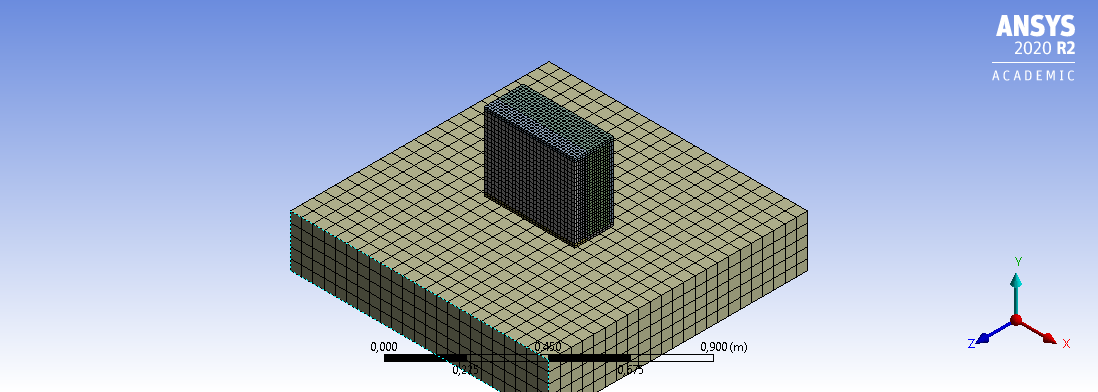
\includegraphics[width=1\textwidth]{figuras/estrutura_simulacaoImpacto/maletaMalha.png}
	\caption{Malha da maleta da estação de controle}
	\label{malha_maleta}
	\end{figure}

\begin{figure}[H]
	\centering
		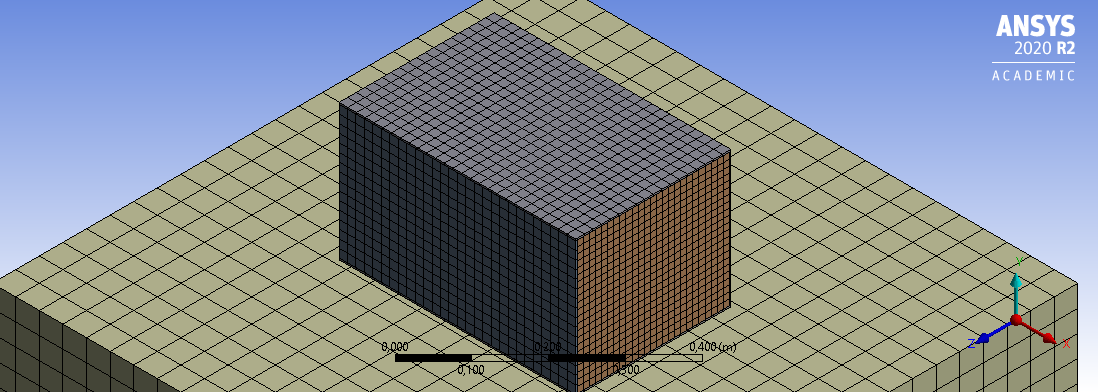
\includegraphics[width=1\textwidth]{figuras/estrutura_simulacaoImpacto/ignicaoRevestidaMalha.png}
	\caption{Malha da maleta do sistema de alimentação com revestimento}
	\label{malha_igniçãoRevestida}
	\end{figure}

\par Para cada uma das duas maletas (com e sem revestimento), foram simuladas três situações de queda: queda direta, quando a maleta com a face inferior; queda lateral, quando a maleta cai com a face lateral voltada para baixo; e queda inclinada, quando a maleta cai "de quina", com inclinação de 45$^{\circ}$ nos eixos X e Z. Foram colhidos os resultados da tensão normal no sentido do eixo Y, da tensão de cisalhamento no plano XZ e da deformação. A seguir, alguns exemplos de resultados da simulação. Os resultados completos encontram-se no Apêndice \ref{simulacoes_impacto}.

\begin{figure}[H]
	\centering
		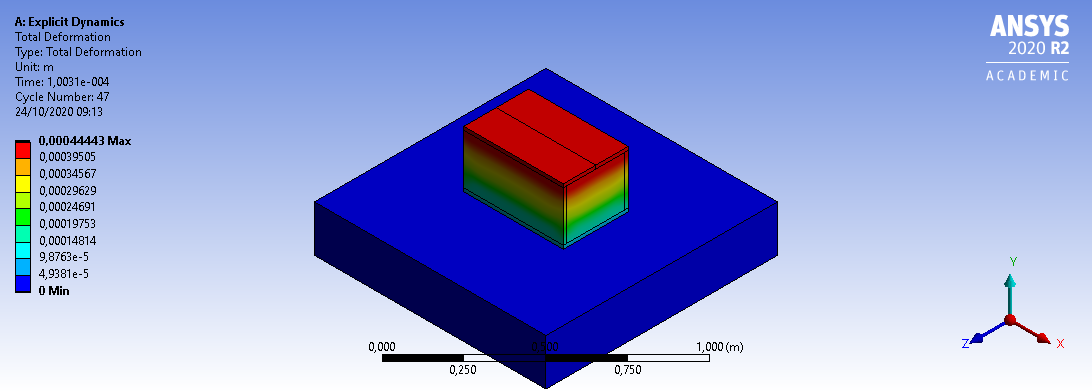
\includegraphics[width=1\textwidth]{figuras/estrutura_simulacaoImpacto/ignicaoDeformacaoLadoMaior.png}
	\caption{Deformação da maleta do sistema de alimentação}
	\label{deformacao_alimentacao1}
	\end{figure}

\begin{figure}[H]
	\centering

		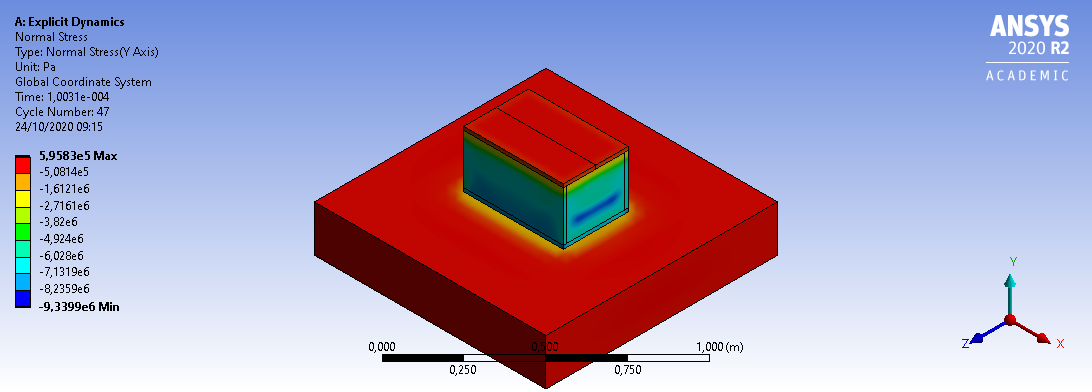
\includegraphics[width=1\textwidth]{figuras/estrutura_simulacaoImpacto/ignicaoNormalYLadoMaior.png}
	\caption{Tensão normal no eixo Y da maleta do sistema de alimentação}
	\label{normal_alimentacao1}
	\end{figure}

\begin{figure}[H]
	\centering

		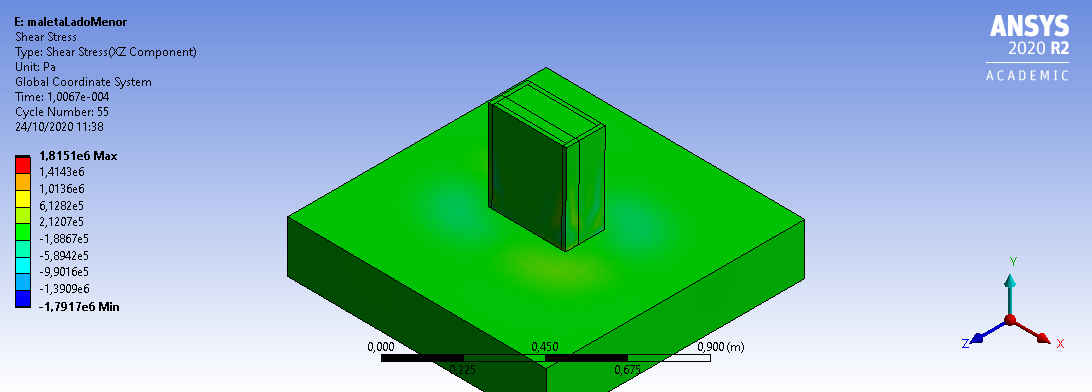
\includegraphics[width=1\textwidth]{figuras/estrutura_simulacaoImpacto/maletaCisalhamentoXZMenor.png}
	\caption{Tensão de cisalhamento no plano XZ da maleta da estação de controle}
	\label{cisalhamento_controle2}
	\end{figure}

\begin{figure}[H]
	\centering

		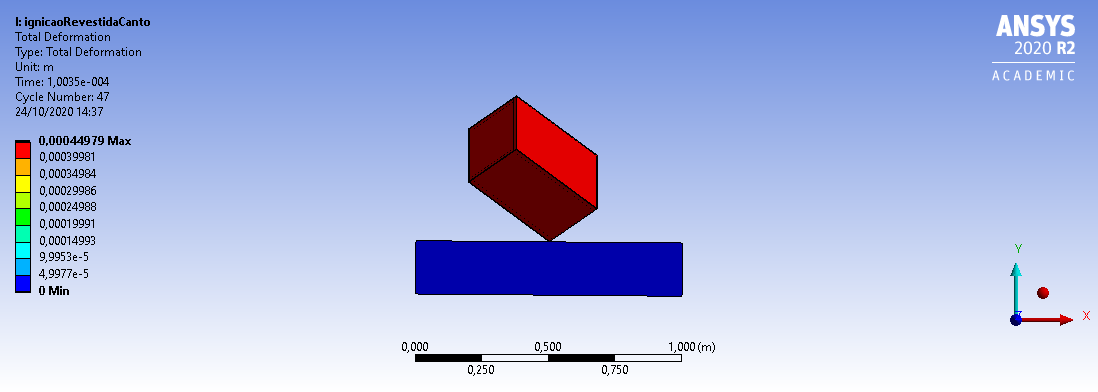
\includegraphics[width=1\textwidth]{figuras/estrutura_simulacaoImpacto/ignicaoRevestidaDeformacaoCanto.png}
	\caption{Deformação da maleta do sistema de alimentação revestida}
	\label{deformacao_alimentacao3}
	\end{figure}

\par A seguir, a tabela com as tensões máximas e mínimas encontradas em cada simulação, as quais são identificadas por qual maleta se refere (sistema de alimentação ou estação de controle), se é tensão normal ou de cisalhamento, e se a queda foi direta, lateral ou inclinada. 

\begin{table}[H]
\centering
\resizebox{\textwidth}{!}{
\begin{tabular}{|l|l|l|}
\hline
Simulação  & Tensão Máxima (MPa) & Tensão Mínima (MPa) \\ \hline
alimentacaoNormalYDireta & $0,59583$ & $-9,3399$ \\ \hline
alimentacaoNormalYLateral & $0,37206$ & $-9,3967$ \\ \hline
alimentacaoNormalYInclinada & $3,3523 $ & $-12,223$ \\ \hline
alimentacaoCisalhamentoXZDireta & $0,81508$ & $-0,81508$ \\ \hline
alimentacaoCisalhamentoXZLateral & $1,9612 $ & $-1,9596 $ \\ \hline
alimentacaoCisalhamentoXZInclinada & $0,26139$ & $-0,38643$ \\ \hline
alimentacaoRevestidaNormalYDireta & $0,028364 $ & $-8,0259 $ \\ \hline
alimentacaoRevestidaNormalYLateral & $2,059    $ & $-7,0118 $ \\ \hline
alimentacaoRevestidaNormalYInclinada & $0,0089829$ & $-0,23426$ \\ \hline
alimentacaoRevestidaCisalhamentoXZDireta & $0,67153$ & $-0,67265  $ \\ \hline
alimentacaoRevestidaCisalhamentoXZLateral & $1,8155  $ & $-1,85    $ \\ \hline
alimentacaoRevestidaCisalhamentoXZInclinada & $0,040217$ & $-0,011293$ \\ \hline
controleNormalYDireta & $0,71074$ & $-10,227$ \\ \hline
controleNormalYLateral & $0,32924$ & $-9,2306$ \\ \hline
controleNormalYInclinada & $3,3956 $ & $-14,927$ \\ \hline
controleCisalhamentoXZDireta & $1,8516$ & $-1,864  $ \\ \hline
controleCisalhamentoXZLateral & $1,8151$ & $-1,7917 $ \\ \hline
controleCisalhamentoXZInclinada & $0,15228$ & $-0,3387$ \\ \hline
controleRevestidaNormalYDireta & $0,28413$  & $-9,2949 $ \\ \hline
controleRevestidaNormalYLateral & $0,14364$  & $-9,1736 $ \\ \hline
controleRevestidaNormalYInclinada & $0,015917$ & $-0,28447$ \\ \hline
controleRevestidaCisalhamentoXZDireta & $1,9844$  & $-2,0515  $ \\ \hline
controleRevestidaCisalhamentoXZLateral & $2,1266$  & $-2,0978  $ \\ \hline
controleRevestidaCisalhamentoXZInclinada & $0,040660$ & $-0,028875$ \\ \hline
\end{tabular}}

\caption{Tensões máximas e mínimas em cada simulação}
\label{tab:ABS}
\end{table}	
	
	
\subsubsection{Plano de construção}

\par Uma vez que os materiais e as dimensões das maletas foram definidos, foi elaborado o passo a passo para a construção destas.

\begin{enumerate}

    \item Primeiro deverá ser feita a parte externa de cada maleta. Para isso as chapas de MDF deverão ser cortadas de acordo com as dimensões externas de cada caixa. Um motor-serra deverá ser utilizado para tal finalidade (ou deverá ser feita a encomenda dos cortes para a empresa fornecedora com as dimensões definidas).
    \item Após isso, será feita a aplicação do material de revestimento nas chapas cortadas. Com o auxilio de cola apropriada para aplicação do material.
    \item O terceiro passo é pregar as chapas de MDF com parafusos e isolar suas quinas com silicone.
    \item O quarto passo é a colocação das partes internas da maleta de suporte. 
    \item Deve-se ainda pensar nas partes destinadas a passagem dos fios elétricos e eletrônicos.  
    \item O último passo é a colocação de dobradiças que conectem as partes, aplicação das alças bem como os protetores de quina.
    
\end{enumerate}

\subsection{Abastecimento}
\label{abastecimento}

\par No presente trabalho, o sistema de abastecimento é todo o conjunto que engloba o sistema de alimentação e os processos necessários para que o oxidante líquido seja transferido para o foguete de forma remota, segura e no momento indicado pelo usuário. Pode-se ainda citar os processos ocorridos para a ignição como apresentado em \ref{sec:ignição}. 

\subsubsection{Fluxo de trabalho}

\par A seguir é apresentado um fluxograma do sistema de alimentação, figura \ref{fig:sistema de alimentacao}. Logo em seguida é caracterizado os componentes do sistema, desde os pré estabelecidos pelo cliente, até os definidos pelo grupo.

\begin{figure}[H]
\centering
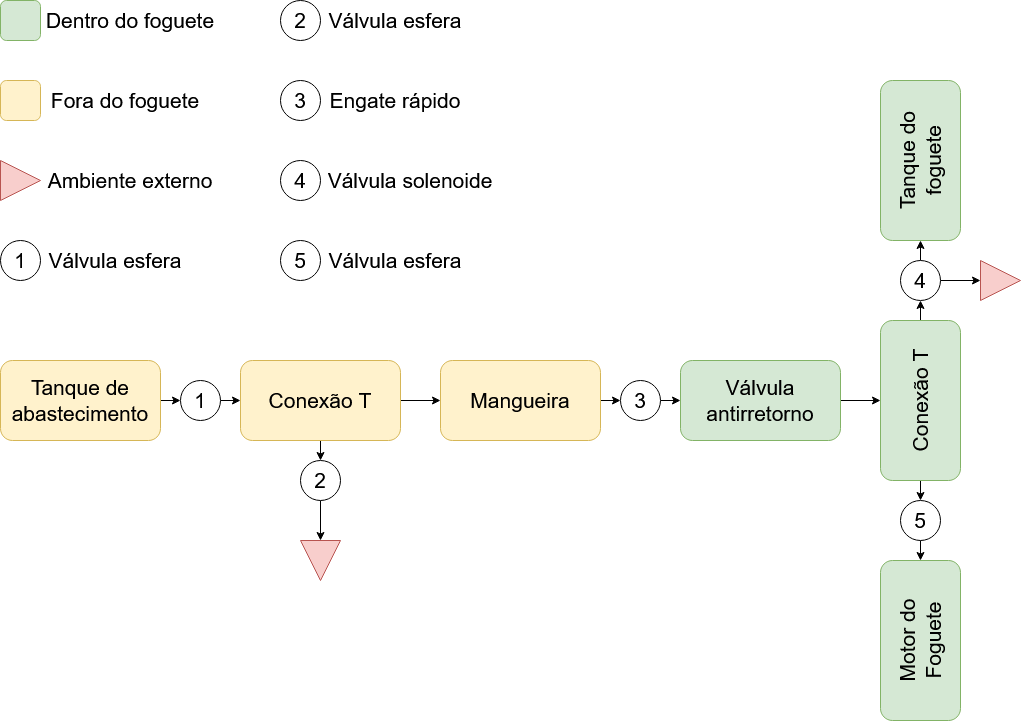
\includegraphics[width=0.9\textwidth]{figuras/diagramaAlimentacao}
\caption{Fluxograma do sistema de alimentação}
\label{fig:sistema de alimentacao}
\end{figure}


\par Com base no projeto desenvolvido pelo cliente \cite{capitalrocketteam2020}, o funcionamento do sistema de abastecimento ocorre em etapas, cada uma delas correspondendo ao estados das válvulas, se estão abertas ou fechadas conforme a ação desejada, figura \ref{fig:sistema de alimentacao}. 

\begin{enumerate}
    \item \textbf{Etapa 1 - Estado inicial}: todas as válvulas estarão fechadas, ou seja, o sistema estará em repouso, de modo a evitar qualquer vazamento antes do início do processo de abastecimento; 
    
    \item \textbf{Etapa 2 - Resfriamento do tanque do foguete}: abertura das válvulas 1 e 4, de modo a realizar a passagem de um fluxo inicial do fluido oxidante, com a finalidade de resfriar o tanque do foguete e otimizar seu abastecimento. O tempo de resfriamento fica a critério do usuário, e a etapa é encerrada com o fechamento das duas válvulas;
    
    \item \textbf{Etapa 3 - Abastecimento do tanque}: abertura da válvula 1, com posterior abertura e fechamento intermitente da válvula 4 para alívio da pressão interna do tanque do foguete durante seu abastecimento. O fluido oxidante é transportado, devido a fenômenos termodinâmicos, em estado de mistura (líquido e gás), e no tanque do foguete a sua fase gasosa deverá ser expulsa pela válvula 4, até o nível definido pelo usuário, este é controlado pela célula de carga que mede a variação de peso do foguete. Com base nos dados fornecidos pela célula de carga, o usuário avaliará se o tanque se encontra cheio, encerrando a etapa com o fechamento da válvula 1 e, caso aberta, da válvula 4; 
    \item \textbf{Etapa 4 - Alívio de pressão da mangueira}: abertura da válvula 2 para expurgo do fluido oxidante que se encontra no interior da mangueira, de modo a equalizar sua pressão interna com a pressão ambiente, de modo a ser possível realizar seu desacoplamento do foguete. A existência de uma válvula anti-retorno na linha de abastecimento impede que o fluido contido no tanque do foguete seja também expurgado nessa fase; 
    \item \textbf{Etapa 5 - Desacoplamento da mangueira}: acionamento do engate rápido, por meio de um atuador linear, de modo a desacoplar e afastar a mangueira do foguete. Essa etapa encerra o processo de abastecimento, e o foguete está preparado para o lançamento; 
    \item \textbf{Etapa 6 - Ignição do foguete}: após o acionamento do ignitor junto ao combustível no motor do foguete, por meio do comando da estação de controle, é feita a abertura da válvula 5, que injetará o fluido oxidante do tanque do foguete na câmara de combustão no interior do motor. Assim o encontro desse fluido com o combustível e o calor gerado pelo ignitor iniciará a combustão principal, e o foguete iniciará sua decolagem.
\end{enumerate}

\par Como mencionado, durante o transporte do fluido oxidante do tanque de abastecimento para o tanque do foguete, fenômenos termodinâmicos ocorrem, como a queda de temperatura provocada pela passagem do fluido conforme ele vai reduzindo a pressão à qual estava submetido no cilindro comercial (por volta de 50 bar). Em alguns casos, esse fenômeno é desejável, como para o resfriamento do tanque do foguete, em outros, ele pode apresentar um problema, como o congelamento de válvulas e atuadores que não estejam nas especificações adequadas. Do mesmo modo, a atuação das válvulas ocorrerá em situações em que o fluido estará a grande pressão, o que impede o manuseio delas manualmente, seja por necessidade, seja por questões de segurança. Ademais, não é recomendado o uso de mangueiras muito longas para o abastecimento, devido à perda do fluido durante seu transporte.

\par A solução proposta é o acoplamento de dois atuadores rotativos nas válvulas 1 e 2, os quais receberão um comando remoto de abertura e fechamento a partir da estação de controle. Para tanto, será necessário tanto o dimensionamento das opções comerciais para atuadores, desde o torque gerado por cada um dos modelos até sua natureza – se eletrônico ou pneumático, quanto o desenvolvimento de uma estrutura de suporte e adaptação entre esses atuadores e as válvulas e conexões do sistema de alimentação, a qual também deverá observar as características (variação de temperatura e pressão) do processo der abastecimento.

\par Deve-se atentar ao fato de que o cliente pediu uma mudança de escopo onde ficou decidido que o dispositivo mecânico responsável pelo desacoplamento e remoção física da mangueira do foguete, a etapa 5 do sistema, representado por 3 na figura \ref{fig:sistema de alimentacao},  será desenvolvido por eles. Cabendo à equipe apenas desenvolver a solução responsável por enviar o comando de desengate a partir da estação de controle. Eles ainda demandaram que esse sistema será baseado em um servo motor ou um motor como usado pelo grupo na solução de válvulas.

\subsubsection{Caracterização dos componentes}

\par Nessa seção estão apresentadas as características especificas dos componentes do sistema de abastecimento.

\begin{itemize}

    \item \textbf{Tanque de abastecimento}: É um cilindro comercial fornecido pela empresa distribuidora de óxido nitroso. A válvula esfera, item 1 da figura \ref{fig:sistema de alimentacao}, deverá ser conectada no bocal de saída desse cilindro, com uso de adaptador caso necessário.
    \par Informações Técnicas: Cilindro de aço para 10 litros ou 7,0 Kg de óxido nitroso; Altura: 70 cm;    Diâmetro: 20 cm; Peso aproximado: 15 Kg.
    
    \item \textbf{Válvula esfera macho-fêmea 1/2 polegada NPT}: É uma válvula de abertura de 90$^{\circ}$. Seu manipulo deverá ser retirado e a haste ligada à esfera de abertura/fechamento será conectada ao mecanismo eletromecânico de abertura. 
     \par Informações Técnicas: Anexo \ref{valvula}
    
    \item \textbf{Conector em T macho-fêmea-macho 1/2 polegada NPT}: São adaptadores em pontos de bifurcação do sistema hidráulico.
    \par Informações Técnicas: para conexões pneumáticas os Tee e cotovelos são forjados em latão, Liga UNS - C37700 - TM, que proporcionam maior dureza e resistência contra golpes, choques mecênicos e vibrações, com absoluta inexistência de porosidade e trincas. A pressão de trabalho precisa ser compatível com as especificações do tubo utilizado.
    
    \item \textbf{Tubo flexível 1/2 polegada de aço inox com tramas de aço}: É necessário por não reagir com o óxido nitroso, como ocorre com a borracha, comum nas mangueiras convencionais.
    
    \item \textbf{Engate rápido 3/4 polegada NPT}: É uma conexão composta por duas peças (macho e fêmea) e um anel de segurança. Somente movendo o anel é que as duas peças podem ser desconectadas.
    
    \item \textbf{Válvula anti-retorno macho-fêmea 3/4 polegada NPT}: É uma válvula de sentido único, ligada ao engate rápido da mangueira e o conector T que liga o tanque ao motor dentro do foguete. Evita que o óxido nitroso volte no sentido do tanque de abastecimento.
    
\end{itemize}   

 
\par No anexo \ref{ane:Elementos do sistema de alimentação} é apresentada mais informações técnicas de cada um dos elementos descritos nessa seção.

\subsubsection{Atuador}

\par O dimensionamento do atuador exige conhecimento do torque necessário para abrir a válvula esfera. Um estudo feito por Silva, aponta que o torque inicial necessário para abrir uma válvula esfera sob pressão de óxido nitroso é de 2 N.m.
\par Assim a solução para a abertura e fechamento de válvulas por comando remoto é a utilização de um motor de 12 Volts acoplado com um sistema de caixa redutora conectado a válvula. O sistema de caixa redutora possui a função de aumentar o torque do motor elétrico, diminuindo a velocidade de rotação.
\par A proposta é utilizar um motor de para-brisa que já possui uma caixa redutora acoplada a ele. 

\par O óxido nitroso se apresenta em uma mistura líquido-vapor, com pressão de aproximadamente 57 bar a temperatura ambiente de 25$^{\circ}$C. Admitindo uma margem de segurança, decidiu-se impor o critério de que a válvula deve suportar pressões de pelo menos 68 bar e temperaturas mínimas de até -20$^{\circ}$C. 

\par O atuador deve-se ter um torque mínimo que vai depender da válvula a ser utilizada, pode ser pesquisada o torque necessário para abrir a partir de dados do fabricante. No \textit{datasheet} da válvula escolhida é mostrado um torque de aproximadamente 1,5 N.m. e tempo de resposta de aproximadamente 2 segundos. Com base nesse torque, foram selecionadas duas opções
\par O Motor de vidro elétrico de carro: necessita ponte H (~R\$25) para realizar abertura e fechamento. Posição intermediária difícil de se obter, não há precisão na posição do motor. 
\par Informações técnicas: Voltagem 12V; Consumo 1,3A; Força 9,12 N.m / 93Kg.cm; Valor de ~ R\$60.

\par Servo motor Ds3218: consegue ajustar bem a posição, possui um maior controle de vazão. Consumo bem menor que o motor. É mais caro e gera menos torque, precisaria-se de dois servos para cada válvula, para trabalhar com segurança.
\par Informações técnicas: Voltagem 7.2 V; Consumo 100 mA; Força 2,19 N.m / 22.3 Kg.cm; Valor ~ R\$135

\par Assim, a escolha do atuador permeia o subnúcleo de energia, pois os valores de corrente são bem diferentes. Além disso, é necessário delimitar o preço, pois na verdade há no mercado válvulas esferas com atuadores elétricos pronto para uso, entretanto, como a pressão de trabalho é alta e a temperatura é baixa, o fluido no nosso projeto exige uma válvula robusta, que por sua vez exige um motor tão robusto quanto para abrir as válvulas, o custo de uma pronta é muito elevado de ~ R\$1000 cada. 

\par Com isso apresentado, a escolha foi do motor de vidro elétrico de carro que tem seus aspectos técnicos apresentados no anexo \ref{motorcarro}.


\subsubsection{Oxido Nitroso}
\label{sec:n2o}

A escolha do óxido nitroso como parte do par propelente é justificada pelas vantagens que esse gás industrial traz devido às suas características. Como já mencionado, esse gás é auto pressurizante, podendo ser armazenado a altas pressões (por volta de 50bar) a temperatura ambiente (20ºC), o que dispensa a necessidade de sistemas de pressurização e expulsão do tanque para o motor do foguete (necessitando apenas a abertura da válvula para o início da ignição). Além disso, é um gás comercial de fácil aquisição, relativamente barato em comparação a outros propelentes, é não tóxico, facilmente armazenável e de baixa inflamabilidade na ausência de seu par combustível \cite{rogerapazavasquez2017}. 

Abaixo algumas características físico-químicas importantes para o uso dessa substância \cite{rogerapazavasquez2017}: 

\begin{table}[H]
\centering
\begin{tabular}{|l|l|}
\hline
Massa molar & $44,013 kg/mol$ \\ \hline
Ponto de ebulição & $-88,5 ^{\circ}C$  \\ \hline
Ponto de fusão & $-90,8 ^{\circ}C$  \\ \hline
Temperatura crítica & $36,4 ^{\circ}C$ \\ \hline
Pressão crítica & $72,45 bar$  \\ \hline
Pressão de vapor (20 $^{\circ}$C) & $50,8 bar$  \\ \hline
Condutividade térmica (0 $^{\circ}$C) & $14,57 mW/(m.K)$  \\ \hline
Entalpia de formação & $82 kJ/mol$  \\ \hline
\end{tabular}
\caption{Características físico-químicas do óxido nitroso}
\label{tab:n2o}
\end{table}

\par Para fins do presente trabalho, a temperatura do gás é o parâmetro mais importante, uma vez que ela pode afetar o funcionamento do sistema de alimentação. Como dito, o óxido nitroso é armazenado à alta pressão e à temperatura ambiente. Isso significa que, quando é aberta a válvula do cilindro de abastecimento, ocorre uma queda de pressão do gás enquanto ele passa pelo sistema de alimentação, o que incorre numa queda de temperatura brusca, o cliente relatou que experiências passadas mostraram risco de congelamento de válvulas caso estas não fossem capazes de trabalhar a baixas temperaturas. 

\subsubsection{Metodologia}

\par A simulação do sistema de abastecimento foi feita no software \textit{Simulink/Matlab} pois se trata de uma ferramenta confiável e conhecida no ramo de engenharia. A robustez do software se torna aliada uma vez que possui blocos nativos que representam fisicamente cada um dos componentes, permitindo uma maior agilidade na montagem e modelagem do problema. 

\par O projeto do sistema de alimentação foi desenvolvido usando-se o \textit{Simscape Fluids}, uma ferramenta do \textit{Matlab/Simulink}, onde ele fornece bibliotecas de componentes para modelagem e simulação de sistemas de fluidos, incluindo modelos de bombas hidráulicas, válvulas, atuadores, dutos e trocadores de calor. Para o abastecimento de combustível do foguete iremos usar o componentes de válvulas, atuadores e dutos integrado com as bibliotecas do \textit{Simscape Eletric}, um análogo a aquele para sistemas elétricos. 

\par O uso dessa ferramenta se da pois a mesma ajuda no desenvolvimento de sistemas de controle, onde é possível se testar o desempenho em nível de sistema. Com isso a principal biblioteca utilizada é a de Modelos Hidráulicos, na qual está-se presente os blocos hidráulicos básicos de temperatura constante seguindo-se as técnicas de modelagem apresentadas.

\par A seguir são apresentadas as etapas essenciais para construir e simular um modelo físico de sistema. A figura \ref{fig:metodologia} mostra o passo a passo para esse desenvolvimento.

\begin{figure}[h!]
\centering
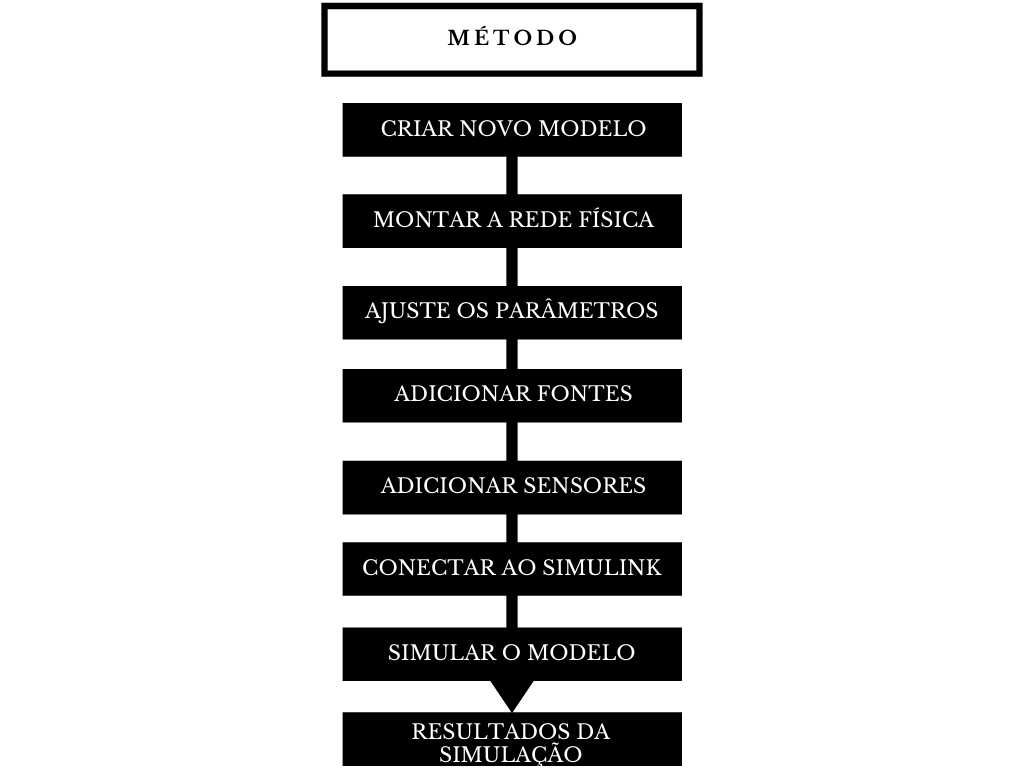
\includegraphics[width=0.9\textwidth]{figuras/metodo.png}
\caption{Etapas de simulação}
\label{fig:metodologia}
\end{figure}

\begin{enumerate}
    \item Etapa 1: Criar um novo modelo 
    \item Etapa 2: Montar a rede física, para modelar o sistema, adiciona-se blocos das bibliotecas \textit{Simscape} a um modelo e, em seguida, os conecta a uma rede física. 
    \item Etapa 3: Ajuste os parâmetros do bloco e as metas variáveis
    \item Etapa 4: Adicionar fontes, definir sinais de entrada.
    \item Etapa 5: Adicionar sensores, para medir as quantidades da rede física. 
    \item Etapa 6: Conectar ao \textit{Simulink} com blocos de interface
    \item Etapa 7: Simular o modelo
    \item Etapa 8: Ver os resultados da simulação
\end{enumerate}


\par A simulação matemática no ambiente do software foi ajustada com os parâmetros da tabela \ref{tab:abas} e os demais, por se tratarem de parâmetros que não alteram significativamente o resultado, foram deixados os valores padrão do programa.

\par Para as propriedades do fluído segue-se o que foi apresentado na seção \ref{sec:n2o}. Assim mesmo o óxido nitroso se apresentando como uma mistura líquido-vapor, com pressão de aproximadamente 57 bar a temperatura ambiente de 25\degree C \cite{Propriedades_termofisicas}, foi assumido que o escoamento do óxido nitroso se dá na fase líquida e a uma temperatura constante. Dado a complexidade de se fazer a modelagem e simulação como um escoamento em duas fases (líquido e vapor), como é o caso real. 

\begin{table}[H]
\centering
\begin{tabular}{|l|l|}
\hline
Densidade do óxido nitroso (a 25\degree C)              & 750 $kg/m^3$ \\ \hline
Viscosidade cinemática (líquido)            & $0,0639 x 10^6  m^2/s$ \\ \hline
Volume de óxido nitroso            & 7  $L$ \\ \hline
Diâmetro das tubulações                      & 2 $cm$ \\ \hline
\end{tabular}
\caption{Parâmetros da simulação de abastecimento}
\label{tab:abas}
\end{table}

\subsubsection{Modelagem matemática}

\par Para a solução do nosso problema é necessária a criação de um adaptador para as válvulas do sistema de abastecimento. Esse sistema tem por objetivo transportar o propelente líquido do tanque de abastecimento para o tanque do foguete. Assim uma simulação que se aproxime do sistema eletromecânico desenvolvido, foi feita como meio de verificar sua usabilidade.

\par A seguir serão apresentados os blocos usados para o nosso sistema.

\begin{itemize}
    \item Caracterização do fluído combustível - \textit{Custom Hydraulic Fluid} 
    \par O primeiro passo é caracterizar o fluido combustível que devera ser transportado, deve-se atentar ao fato de que essas propriedades serão consideradas constantes durante o tempo de simulação. Para o nosso caso o cliente especifica o uso do oxido nitroso, por isso esse é o fluido que trabalharemos aqui, assim suas propriedades são apresentadas na seção \ref{sec:n2o}.
    \par Este bloco atribui propriedades de fluido para todos os componentes montados no \textit{loop}. 
    \par Os parâmetros utilizados são: densidade; viscosidade cinemática (líquido); módulo de compressibilidade, assim se o escoamento for incompressível; quantidade relativa de ar preso.
    \par As variáveis necessárias são: volume do fluido; nível do fluido.
    
    \item Tanque de abastecimento - \textit{Tank}
    \par Cilindro comercial fornecido pela empresa distribuidora do óxido nitroso. A válvula esfera deverá ser conectada no bocal de saída desse cilindro, com uso de adaptador caso necessário. 
    \par O bloco do Simulink indicado possue um sinal de saída que indica o volume de fluido no tanque e um sinal de entrada que é a porta de conservação hidráulica associada à entrada do tanque. A perda de carga pode ser inserida por meio do valor de \textit{pipeline pressure loss coefficient}. 
    \par Tanque com pressão constante, leva em conta a mudança no nível do fluido e por isso é fornecida a área de seção transversal do tanque. 
    \par Os parâmetros necessários são: pressurização; nível do fluido; diâmetro da tubulação de entrada; coeficiente de perda de pressão do duto.
    
    \item Válvula esfera - \textit{Ball Valve} 
    \par Este bloco modela a redução de fluxo devido a uma válvula de esfera em uma rede hidráulica. Possui duas portas hidráulicas sendo uma associada a entrada e outra associada saída da válvula. Possui uma porta de entrada de sinal físico que indica o deslocamento capaz de alterar o fluxo do fluido que passa pela válvula. 
    \par Os parâmetros necessários são: diâmetro da esfera; diâmetro do orifício; coeficiente de descarga; \textit{leakage area}; área interna entre as entradas da válvula.
    \par As variáveis necessárias são: queda de pressão; quociente de vazão.
    
    \item Conexão T - \textit{T-junction} 
    \par O bloco representa uma junção em T que consiste em um trecho principal e uma ramificação que se une ao trecho principal em um ângulo especificado. A junção como uma resistência hidráulica é especificada por seis coeficientes de perda de pressão que caracterizam a relação pressão-vazão para cada conexão possível para o fluxo direto e reverso. O bloco apresenta três entradas/saídas hidráulicas (A, B, A1) que representam o fluxo do fluido. 
    \par Os parâmetros de geometria da válvula são: diâmetro do tubo principal; diâmetro do tubo de ramificação; especificação de transição laminar; razão de pressão de fluxo laminar.
    \par A perda de pressão possui os seguintes coeficientes que podem ser alterados: coeficiente de perda de pressão AB; coeficiente de perda de pressão BA; coeficiente de perda de pressão A-A1; coeficiente de perda de pressão A1-A; coeficiente de perda de pressão A1-B; coeficiente de perda de pressão B-A1
    
    \item Ambiente externo - \textit{Hydraulic Reference} \par O bloco de referência hidráulica representa uma conexão com a pressão atmosférica. O bloco possui apenas uma porta de conservação hidráulica.
    
    \item Mangueira - \textit{segmented Pipeline}
	\par Este bloco representa a perda de pressão do fluido em tubulações hidráulicas com seções transversais circulares como um conjunto de segmentos de tubos idênticos, conectados em série. Cada segmento de tubo leva em consideração as propriedades resistivas, de inércia de fluido e compressibilidade de fluido. Possui duas portas hidráulicas sendo uma associada ao fluxo de entrada e outra associada ao fluxo de saída da tubulação. 
	\par Os parâmetros necessários são: diâmetro interno do tubo; comprimento do tubo; número de segmentos; comprimento equivalente agregado de resistências locais; altura de rugosidade da superfície interna; margem superior do fluxo laminar; margem inferior do fluxo turbulento; tipo de parede de tubo; coeficiente de pressão estática de diâmetro; constante de tempo do processo viscoelástico; relação de calor específico; pressões iniciais nos nós do modelo; pressão inicial; vetor de pressão inicial; taxa de fluxo inicial.
	
	\item Válvula anti-retorno - \textit{Check Valve}
	\par Este bloco representa uma válvula de retenção hidráulica com o objetivo de permitir o fluxo em uma direção e bloqueá-lo na direção oposta. A válvula permanece fechada enquanto a diferença de pressão através da válvula é inferior à pressão de abertura da válvula. Quando a pressão de abertura é atingida, o membro de controle de fluxo é forçado a sair de sua sede, criando assim uma passagem entre a entrada e a saída. Se vazão e pressão forem altas o suficiente, a área é aumentada ainda mais até que o membro de controle alcance sua máxima abertura. Possui duas portas hidráulicas sendo uma associada ao fluxo de entrada e outra associada ao fluxo de saída da válvula. 
	\par Os parâmetros necessários são: área máxima de passagem; pressão de fissura; pressão máxima de abertura; coeficiente de vazão; especificação de transição laminar; razão de pressão de fluxo laminar; número crítico de Reynolds; área de vazamento; dinâmica de abertura; constante de tempo de abertura; área inicial;

\end{itemize}

\begin{figure}[H]
\centering
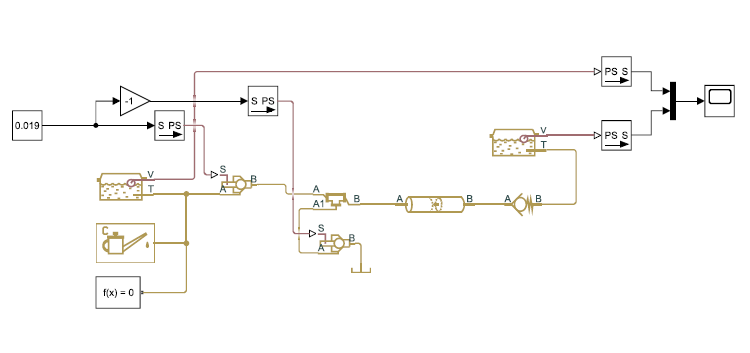
\includegraphics[width=1\textwidth]{figuras/diagrama_hidraulico.png}
\caption{Diagrama hidráulico}
\label{fig:metodologia}
\end{figure}

\begin{figure}[H]
\centering
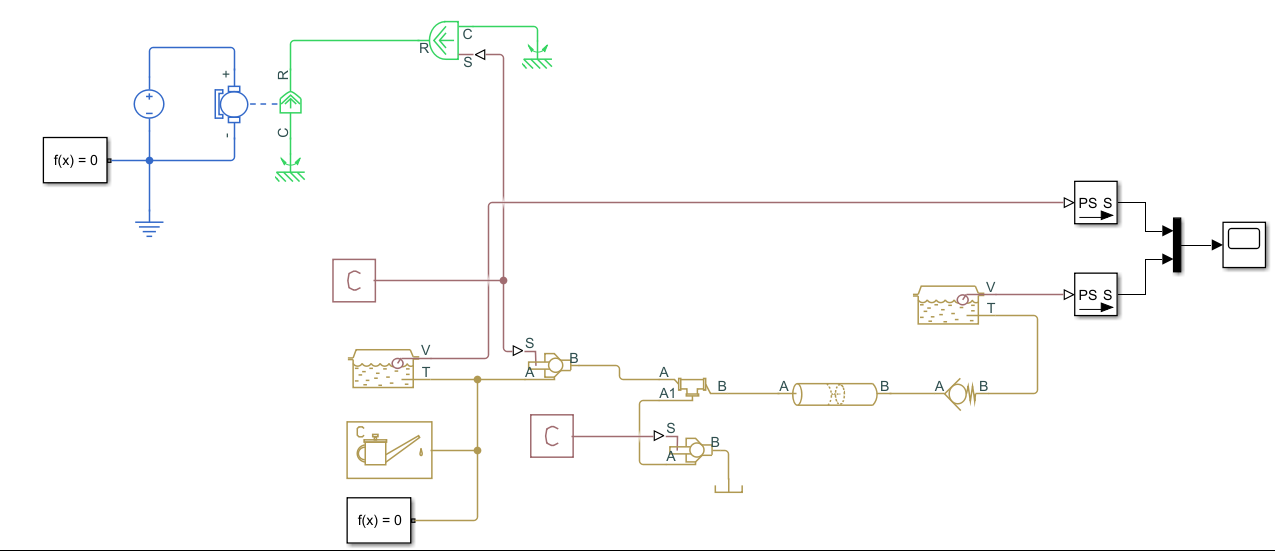
\includegraphics[width=1\textwidth]{figuras/diagrama_mecanico.png}
\caption{Diagrama eletromecânico}
\label{fig:metodologia}
\end{figure}

